\documentclass[../../main.tex]{subfiles}

\begin{document}

\chapter{Quantum many-body framework}

This chapter is dedicated to introducing the necessary tools needed to perform realistic material calculations using DMFT or D$\Gamma$A. We start with the most central objects - the Green's functions - and subsequently assemble a complete framework which enables us to calculate a number of physical properties, e.g. the susceptibility, optical conductivity, superconductivity, pseudogaps and more, that stem from the correlated interplay between electrons or holes. 

\section{One-particle Green's functions}

Green's functions are fundamental tools in many-body physics, used to study the properties and behavior of interacting quantum systems. These mathematical objects encode information about the propagation of particles or excitations within a system and serve as the cornerstone for analyzing both equilibrium and nonequilibrium states. In the many-body regime, Green's functions extend beyond single-particle descriptions to include complex interactions among multiple particles. They provide insights into phenomena such as quasiparticle lifetimes, collective excitations and response functions. Specifically, one- and two-particle Green's functions describe the propagation of a single particle and the correlated motion of particle pairs, respectively. Alongside of the mathematical description of Green's function-based expressions, we also provide a pictorial description of the equations using Feynman diagrams. These Feynman diagrams allow us to easily describe interaction processes visually. Lines and vertices within the diagrams indicate particle propagators and interaction vertices, respectively. External legs will be coloured gray while inner legs and interaction lines will be coloured black.

In condensed matter physics, we are only interested in finite-temperature effects. Hence it is practical to use the so-called Matsubara formalism\cite{T. Matsubara. “A new approach to quantum-statistical mechanics”} in imaginary time by performing a Wick rotation $t\to -i\tau$\cite{G. C. Wick. “Properties of Bethe-Salpeter Wave Functions”}.

Furthermore, most many-body quantities described in the following are $n$-point (correlation) functions\footnote{Here, $n$ denotes the number of \say{external legs} of the corresponding Feynman diagram.}. These functions typically include a subset of the following parameters for each external leg: (Matsubara) frequency ($\nu$), spin index ($\sigma$), orbital index ($o$), lattice position ($\vv{R}$), momentum ($\vv{k}$) or imaginary time ($\tau$). This introduces a huge amount of dependencies appended to a variable and can be very cumbersome to read through if explicitly written down. Therefore, to increase readability, we follow Ref.~\cite{N. E. Bickers and D. J. Scalapino. “Conserving approximations ...”} and group all indices that are not explicitly written down into a compound index, e.g. $\mathfrak{i}=\{o_i, \sigma_i, \vv{R}_i\}$. If an equation containing spatial or momentum-dependent quantities is written down with a compound index, it applies equally in both real and Fourier space. Furthermore, summing over these compound indices means summing over all individual components they include, with a normalization of $\frac 1\beta$ for frequency sums and $\frac{1}{N_{\vv{k}}}$ for momentum sums, where $\beta=\frac{1}{k_B T}$ is the inverse temperature and $N_{\vv{k}}$ is the total number of reciprocal lattice points. 
\\\\
After this short introduction, let us dive in by defining the most central quantity, the two-point (one-particle) Green's function, in a system in thermal equilibrium as
\begin{align}\label{eq:one_p_green_expectation_val}
	G_{\mathfrak{12}}^{\vv{k}}=-\mean{\mathcal{T}\left [\hat{c}_{\vv{k};\mathfrak{1}}\hat{c}^{\dagger}_{\vv{k};\mathfrak{2}}\right ]},
\end{align}
where $\hat{c}_{\vv{k};\mathfrak{i}}$ ($\hat{c}^{\dagger}_{\vv{k};\mathfrak{i}}$) are fermionic annihilation (creation) operators which annihilate (create) an electron with parameters $\mathfrak{i}=\{\sigma_i, o_i, \tau_i\}$ and momentum $\vv{k}$ in the system. $\mean{\cdot}=\frac{1}{Z}\trace{e^{-\beta\hat{\mathcal{H}}}\;\cdot }$ with $Z=\trace{e^{-\beta\hat{\mathcal{H}}}}$ describes the thermal expectation value. Note, that the time evolution operator $e^{i\hat{\mathcal{H}}t}=e^{\hat{\mathcal{H}}\tau}$ is real after performing the Wick rotation to imaginary time and the Boltzmann weight $e^{\beta\hat{\mathcal{H}}}$ describes nothing more than an additional evolution in imaginary time. Lastly, $\mathcal{T}[\cdot]$ is the imaginary time ordering operator, where
\begin{align}
	\mathcal{T}\left [\hat{c}^{(\dagger)}_{\mathfrak{1}}(\tau_1)\hat{c}^{(\dagger)}_{\mathfrak{2}}(\tau_2)\right ]=\Theta(\tau_1-\tau_2)\hat{c}^{(\dagger)}_{\mathfrak{1}}(\tau_1)\hat{c}^{(\dagger)}_{\mathfrak{2}}(\tau_2)-\Theta(\tau_2-\tau_1)\hat{c}^{(\dagger)}_{\mathfrak{2}}(\tau_2)\hat{c}^{(\dagger)}_{\mathfrak{1}}(\tau_1).
\end{align}
The Green's function measures the probability amplitude of a propagation process and reads as a Feynman diagram
\begin{figure}[ht!]
	\centering
	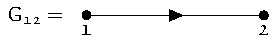
\includegraphics[scale=1.4]{../../Graphics/Diagrams/one_p_green/one_p_green}.
	\caption{Diagrammatic representation of the one-particle Green's function $G_{\mathfrak{12}}$. The electron is annihilated at $\mathfrak{1}$, propagates in imaginary time from $\tau_1$ to $\tau_2$ and is created at $\mathfrak{2}$.}
	\label{fig:one_p_green}
\end{figure}

In homogeneous systems, e.g., infinite or translationally invariant systems, the Green's function inherits the system's properties and becomes invariant under spatial translations. This means that $G_{\mathfrak{12}}(\vv{R}_1, \vv{R}_2)=G_{\mathfrak{12}}(\vv{R}_1-\vv{R}_2,\vv{0})=G_{\mathfrak{12}}(\vv{R})$. In Fourier space, this means that the Green's function is also only dependent on a single momentum parameter, $G_{\mathfrak{12}}(\vv{k}_1, \vv{k}_2)=G_{\mathfrak{12}}(\vv{k}_1-\vv{k}_2,\vv{0})=G_{\mathfrak{12}}(\vv{k})$. Furthermore, if the system is stationary, i.e., the Hamiltonian is not explicitly dependent on imaginary time, then $G_{\mathfrak{12}}(\tau_1, \tau_2)=G_{\mathfrak{12}}(\tau_1-\tau_2,0)=G_{\mathfrak{12}}(\tau)$. In absence of spin-orbit coupling, the spins at $\mathfrak{1}$ and $\mathfrak{2}$ need to be equal and therefore $G_{\mathfrak{12}}$ only depends on a single spin component. Additionally, the \textit{fermionic} Green's function can be shown to be anti-periodic in imaginary time with a period of $\beta$\footnote{This originates from the Boltzmann term $e^{\beta\hat{\mathcal{H}}}$ in the thermal expectation value and restricts the imaginary time domain to $\tau\in[-\beta,\beta)$.},
\begin{subequations}
\begin{align}
	G_{\mathfrak{12}}(\tau)&=-G_{\mathfrak{12}}(\beta-\tau)\quad\text{for } \tau>0 \text{ and}\\
	G_{\mathfrak{12}}(\tau)&=-G_{\mathfrak{12}}(\beta+\tau)\quad\text{for } \tau<0.
\end{align}
\end{subequations}
This anti-periodicity in time leads to the Fourier transform to be defined over a discrete set of imaginary frequencies, the the so-called Matsubara frequencies, which for fermionic quantities are given by $\nu_n=(2n+1)\frac\pi\beta$. In contrast, \textit{bosonic} Green's functions are periodic in imaginary time with period $\beta$ and therefore the Fourier transform includes the set of bosonic Matsubara frequencies $\omega_n=(2n)\frac\pi\beta$. In the following, we will always denote fermionic Matsubara frequencies with $\nu_n$ and bosonic ones with $\omega_n$. The fermionic- and bosonic-like Fourier transforms of $G_{\mathfrak{12}}(\tau)$ become, respectively,
\begin{align}
	G_{\mathfrak{12}}(i\nu_n)=\integral{0}{\beta}{\tau}G_{\mathfrak{12}}(\tau) e^{i\nu_n\tau} \quad\text{and}\quad G_{\mathfrak{12}}(i\omega_n)=\integral{0}{\beta}{\tau}G_{\mathfrak{12}}(\tau) e^{i\omega_n\tau}
\end{align}
and only require the knowledge of Green's functions for positive imaginary times $\tau$. The inverse Fourier transforms are given by
\begin{align}
	G_{\mathfrak{12}}(\tau)=\frac1\beta \sum_n G_{\mathfrak{12}}(i\nu_n) e^{-i\nu_n\tau} \quad\text{and}\quad G_{\mathfrak{12}}(\tau)=\frac1\beta \sum_n G_{\mathfrak{12}}(i\omega_n) e^{-i\omega_n\tau}.
\end{align}
If we perform a spectral representation of the fermionic Green's function in \eqref{eq:one_p_green_expectation_val} and calculate the discrete Fourier transform, we find that
\begin{align}
	G_{\mathfrak{12}}(i\nu_n)=\frac1Z\sum_{mn}\left (e^{-\beta E_n}+e^{-\beta E_m}\right )\frac{\sandwich{n}{\hat c_{\mathfrak{1}}}{m}\sandwich{m}{\hat c^{\dagger}_{\mathfrak{2}}}{n}}{i\nu-(E_m-E_n)}.
\end{align}
If we take $\mathfrak{1}\equiv \mathfrak{2}$, which corresponds to the \textit{local} Green's function, we can introduce the spectral function
\begin{align}
	A_{\mathfrak{1}}(\nu)=\frac1Z\sum_{mn} e^{-\beta E_n}\left (1+e^{-\beta\nu}\right ) |\sandwich{n}{\hat c_{\mathfrak{1}}}{m}|^2 \delta(\nu-E_m-E_n),
\end{align}
where,
\begin{align}
	G_{\mathfrak{1}}(i\nu_n)=\integral{\mathbb{R}}{}{\nu}\frac{A_{\mathfrak{1}}(\nu)}{i\nu_n-\nu}.
\end{align}
The spectral function $A_{\mathfrak{1}}(\nu)$ is the probability of adding or removing a particle with momentum $\vv{k}_1$ with spin $\sigma_1$ from the system. For that reason, $A_{\mathfrak{1}}(\nu)$ is coined the single-particle local density of states. Furthermore, since it represents a probability distribution, the integral over all energies of $A_{\mathfrak{1}}(\nu)$ is equal to $1$. It is directly measurable using techniques like angle-resolved photoemission spectroscopy (ARPES), which probes electronic states in the material and reveals electronic structure properties, such as band gaps and quasiparticle dispersions. The peaks in $A_{\mathfrak{1}}(\nu)$ correspond to quasiparticle states, with their position indicating the energy of these states and their width related to the lifetime or decay rate of the quasiparticles. A narrow peak indicates a well-defined quasiparticle with a long lifetime and weak decay rate, while a broad peak suggests the contrary. The spectral function is a key quantity in many-body theory as it connects real-world experimental results to the Green's function formalism, as is shown in the following. By performing analytic continuation in the upper complex plane ($i\nu\to\nu+i0^{+}$), one can define the retarded Green's function as
\begin{align}
	G_{\mathfrak{1}}^{R}(\nu)=\integral{\mathbb{R}}{}{\nu'}\frac{A_{\mathfrak{1}}(\nu')}{\nu-\nu'+i 0^{+}},
\end{align}
from where one obtains through the Kramers-Kronig relations
\begin{align}
	A_{\mathfrak{1}}(\nu) = -\frac1\pi \Im G_{\mathfrak{1}}^{R}(\nu).
\end{align}
Thus, the spectral function is directly coupled to the imaginary part of the retarded Green's function, connecting many-body theory with physical experiments.

As an example, which will prove itself useful for the future, let us consider non-interacting electrons in a system with translational symmetry that are described by the (Wannier) Hamiltonian
\begin{align}
	\hat{\mathcal{H}}_0=\sum_{\vv{k};\mathfrak{12}}\varepsilon_{\mathfrak{12}}(\vv{k})\hat c^{\dagger}_{\vv{k};\mathfrak{1}}\hat c_{\vv{k};\mathfrak{2}},
\end{align}
where $\varepsilon_{\mathfrak{12}}(\vv{k})=-\sum_{\vv{R};\mathfrak{12}} t_{\mathfrak{12}}(\vv{R})e^{i\vv{kR}}$ is the momentum dispersion of the band and is measured with respect to the chemical potential $\mu$. In this case, it is easy to show, that 
\begin{align}\label{eq:non_interacting_one_p_green}
	G_{0;\mathfrak{12}}(\nu_n, \vv{k})=[i\nu_n\delta_{\mathfrak{12}}-\varepsilon_{\mathfrak{12}}(\vv{k})]^{-1}.
\end{align}
For the one-particle spectral function, we find in this case 
\begin{align}
	A_{\mathfrak{12}}(\varepsilon,\vv{k})=\delta(\varepsilon-\varepsilon_{\vv{k};\mathfrak{12}}),
\end{align}
corresponding to stable quasiparticles, due to zero width of the quasiparticle peak of $A_{\mathfrak{12}}(\varepsilon,\vv{k})$.

The direct computation of the Green's function as expressed in \eqref{eq:one_p_green_expectation_val} generally incurs an exponential increase in cost with lattice size for interacting models. As a result, it is common practice to begin with the noninteracting case and construct a perturbative expansion in terms of the interaction around it. In this context, we will start with the non-interacting case described above. This perturbation expansion will not be derived in detail in this thesis, as there are many wonderful resources that explain it thoroughly \cite{something}, thus we will only sketch it here. In essence, the expansion is constructed using the $S$-matrix and employs strategies such as the Wick contraction \cite{wick contraction} and the linked cluster theorem \cite{linked cluster}. The expansion begins by identifying the most general interaction part of the Hamiltonian of \eqref{eq:general_hubbard_hamiltonian},
\begin{align}
	\hat{\mathcal{H}}_{\text{I}} = \frac12 \sum_{\mathfrak{1234}}U_{\mathfrak{1234}}\hat c^{\dagger}_{\mathfrak{1}}\hat c^{\dagger}_{\mathfrak{3}}\hat c_{\mathfrak{4}}\hat c_{\mathfrak{2}}.
\end{align}
The expansion of the Green's function then reads
\begin{align}
	G_{\mathfrak{12}}(\tau)=-\frac{1}{\mean{S(\beta)}_0}\sum_{n=0}^{\infty}\frac{(-1)^n}{n!}\integral{0}{\beta}{\tau_1}\cdots\integral{0}{\beta}{\tau_n}\mean{\mathcal{T}\left [\hat{c}_{\mathfrak{1}}\hat{c}^{\dagger}_{\mathfrak{2}}\hat{\mathcal{H}}_{\text{I}}(\tau_1)\cdots \hat{\mathcal{H}}_{\text{I}}(\tau_n) \right ]}_0,
\end{align}
where $S(\beta)$ is the abovementioned $S$-matrix and $\mean{\cdot}_0$ is the thermal expectation value in terms of the non-interacting Hamiltonian $\hat{\mathcal{H}}_0$. 
In Feynman diagram jargon, this contains all diagrams that are possible, also disconnected ones\footnote{Disconnected means, that the term includes a diagram that consists of two separate, disconnected diagrams.}. The linked cluster theorem allows us to get rid of those disconnected contributions by effectively cancelling with the $\frac{1}{\mean{S(\beta)}_0}$ term in front. This results in
\begin{align}\label{eq:one_p_green_full_perturbation_exp}
	G_{\mathfrak{12}}(\tau)=-\sum_{n=0}^{\infty}\frac{(-1)^n}{n!}\integral{0}{\beta}{\tau_1}\cdots\integral{0}{\beta}{\tau_n}\mean{\mathcal{T}\left [\hat{c}_{\mathfrak{1}}\hat{c}^{\dagger}_{\mathfrak{2}}\hat{\mathcal{H}}_{\text{I}}(\tau_1)\cdots \hat{\mathcal{H}}_{\text{I}}(\tau_n) \right ]}_0^{\text{conn}},
\end{align}
where $\mean{\cdot}_0^{\text{conn}}$ now indicates that we only consider connected diagrams in the expansion. We can transform this into a diagrammatic representation by applying Wick contractions, which allow us to collect pairs of creation and annihilation operators to form independent expectation values. In the case of the $n=1$ term in the perturbation expansion of the Green's function,
\begin{align*}
	G_{1;\mathfrak{12}}(\tau)=\sum_{\mathfrak{abcd}}\integral{0}{\beta}{\tau_1}U_{\mathfrak{abcd}}\bigg[&- \mean{\mathcal{T}\left [\hat{c}_{\mathfrak{1}}(\tau)\hat{c}^{\dagger}_{\mathfrak{a}}(\tau_1)\right ]}_0 \mean{\mathcal{T}\left [\hat{c}_{\mathfrak{d}}(\tau_1)\hat{c}^{\dagger}_{\mathfrak{c}}(\tau_1)\right ]}_0 \mean{\mathcal{T}\left [\hat{c}_{\mathfrak{b}}(\tau_1)\hat{c}^{\dagger}_{\mathfrak{2}}(0)\right ]}_0\\
	&+\mean{\mathcal{T}\left [\hat{c}_{\mathfrak{1}}(\tau)\hat{c}^{\dagger}_{\mathfrak{a}}(\tau_1)\right ]}_0 \mean{\mathcal{T}\left [\hat{c}_{\mathfrak{b}}(\tau_1)\hat{c}^{\dagger}_{\mathfrak{c}}(\tau_1)\right ]}_0 \mean{\mathcal{T}\left [\hat{c}_{\mathfrak{d}}(\tau_1)\hat{c}^{\dagger}_{\mathfrak{2}}(0)\right ]}_0\bigg].\numberthis
\end{align*}
The remaining expectation values are nothing more than minus the non-interacting Green's function of \eqref{eq:non_interacting_one_p_green}. Written in Feynman diagrams, the first relevant perturbation expansion term is shown in \figref{fig:one_p_green_first_perturbation_term}.
\begin{figure}[ht!]
	\centering
	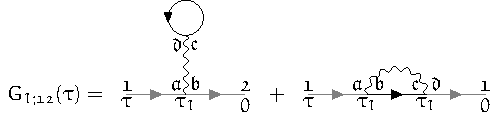
\includegraphics[scale=1.4]{../../Graphics/Diagrams/one_p_green_first_perturbation_term/one_p_green_first_perturbation_term}
	\caption{First order diagrams for the single-particle Green's function. The corresponding diagrams are coined the Hartree- and the Fock-term, respectively. As the name suggests, taking only these two diagrams as the whole perturbation expansion leads to the Hartree-Fock approximation, formulated as a diagrammatic theory.}
	\label{fig:one_p_green_first_perturbation_term}
\end{figure}

\section{Self-energy}

The one-particle Green's function perturbative expansion is already much simplified in the graphical portrayal. However, the number of diagrams increases exponentially with order $n$\footnote{For $n=2$ there exist $10$ diagrams, for $n=7$ the number of diagrams is well over a million.}. Therefore, the Feynman diagram approach would be of little practical use if the only way to progress was to calculate each diagram one at a time. However, in reality the technique is actually quite useful, since it hints on how to sum up the perturbative series. Let us talk about how it applies to Green's function for single particles. First, let us define another compound index which will further levitate readability. We will set $\k=\{\nu,\vv{k}\}$ and $\q=\{\omega, \vv{q}\}$ as a compound index including momentum and frequency in one index for fermionic ($\k$) and bosonic ($\q$) frequencies and momenta. Note, that if we write $\nu$ instead of $\k$, we refer to the \textit{local} part of the quantity with $\vv{k}=\vv{0}$ instead of the \textit{non-local} part.

Diagrams in general can be split up into two classes: (i) diagrams that, by cutting a single internal Green's function line, transform in two lower-order diagrams, which are called one-particle reducible and (ii) diagrams that are not one-particle reducible, which are called one-particle irreducible (1PI). Let us define as the one-particle self-energy $\Sigma_{\mathfrak{12}}^{\k}$ the sum of all irreducible diagrams without external legs. For example, the black part of the diagrams in \figref{fig:one_p_green_first_perturbation_term} corresponds to the first-order diagrams of the self-energy. It is then straightforward to rewrite \eqref{eq:one_p_green_full_perturbation_exp} in terms of the self-energy, yielding
\begin{align}\label{eq:dyson_eq}
	G_{\mathfrak{12}}^{\k}=G_{0,\mathfrak{12}}^{\k}+\sum_{\mathfrak{ab}}G_{0,\mathfrak{1a}}^{\k}\Sigma_{\mathfrak{ab}}^{\k}G_{\mathfrak{b2}}^{\k},
\end{align}
which results in - when taking \eqref{eq:non_interacting_one_p_green} as the noninteracting Green's function and inverting in frequency and momentum space - a way to express the full (interacting) single-particle Green's function in terms of the self-energy
\begin{align}
	G_{\mathfrak{12}}^{\k} = \left [i\nu_n\delta_{\mathfrak{12}}-\varepsilon_{\mathfrak{12}}(\vv{k})-\Sigma_{\mathfrak{12}}^{\k}\right ]^{-1}.
\end{align}
\eqref{eq:dyson_eq} is commonly known as the Dyson equation \cite{dyson eq} for the single-particle Green's function and for completeness, its diagrammatic representation can be found in \figref{fig:dyson_eq}. It is a geometric series, where each term in the sum subsequently adds irreducible diagrams that are pieced together by non-interacting Green's functions to generate all possible diagrams.
\begin{figure}[ht!]
	\centering
	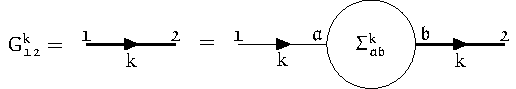
\includegraphics[scale=1.4]{../../Graphics/Diagrams/dyson_eq/dyson_eq}
	\caption{Diagrammatic representation of \eqref{eq:dyson_eq}. The full Green's function $G_{\mathfrak{12}}^{\k}$ is drawn as a thick black line.}
	\label{fig:dyson_eq}
\end{figure}
The self-energy can be obtained by simply inverting \eqref{eq:dyson_eq},
\begin{align}
	\Sigma_{\mathfrak{12}}^{\k}=(G_{0;\mathfrak{12}}^{\k})^{-1}-(G_{\mathfrak{12}}^{\k})^{-1}.
\end{align}
Thus, perturbation theory can be done in two distinct ways: the simpler approach is to determine the Green's function directly, for example, up to order $n$, where the second method is to compute the self-energy up to order $n$ and insert its expression in the Dyson equation \eqref{eq:dyson_eq}. This gives an approximate Green's function containing each order of perturbation theory with only a subset of all possible diagrams. As a result, \eqref{eq:dyson_eq} represents a way to sum up perturbation theory and is actually more relevant from a physical standpoint. Indeed, many methods leverage the usefulness of this approach, for example the dynamical mean-field theory or the dynamical vertex approximation, as we will see later.

Let us add some physical background to the self-energy in the following. $\Sigma$ represents the effects of the interaction on the single electron propagators. The real and imaginary part of the self-energy have significant impact on the physical properties of the system. The real part of the self-energy contributes to an energy shift of the electronic states of the single-particle energy levels $\epsilon(\vv{k})$ due to interactions. In contrast, the imaginary part of the self-energy is related to the decay or lifetime of quasiparticles and introduces a spectral broadening or damping of the electronic states, indicating how long an excitation or quasiparticle persists before interacting with other excitations or scattering events. A larger imaginary part implies a shorter lifetime and stronger interactions. The first order in frequency, $\dpd{\sigma^{\k}}{\nu}$, corresponds to an effective renormalization of the bare electron mass. It also leads to a redistribution of spectral weight in the one-particle spectral function, which provides information about the distribution of energy levels available for excitations. A broader spectral function, whose broadening is controlled by the imaginary part of the self-energy, typically indicates stronger interactions and a more correlated system.

\section{Two-particle Green's functions}

In analogy to the one-particle Green's function, the two-particle Green's function describes the amplitude of the propagation of two particles, two holes or a particle and a hole. A similar expression to \eqref{fig:one_p_green} can be formulated for the two-particle Green's function
\begin{align}
	G_{\mathfrak{1234}}^{\q\k\kp}=-\mean{\mathcal{T}\left [\hat{c}_{\vv{k};\mathfrak{1}}\hat{c}^{\dagger}_{\vv{k}-\vv{q};\mathfrak{2}}\hat{c}_{\vv{k}'-\vv{q};\mathfrak{3}}\hat{c}^{\dagger}_{\vv{k}';\mathfrak{4}}\right ]}.
\end{align}
It describes two particles, two holes or a particle and a hole being inserted in the system at times $\tau_2$ and $\tau_4$, propagating in the system until they are removed again at $\tau_1$ and $\tau_3$, respectively. Assuming a stationary Hamiltonian that satisfies time-translation invariance, it is possible to eliminate one imaginary time variable by setting it zero. Then, the Green's function only depends on three time variables and through Fourier transform, also only depends on three frequency and momentum variables. There are three equivalent choices of independent frequencies (with $\nu$, $\nu'$ being a fermionic and $\omega$ a bosonic Matsubara frequency) 
\begin{subequations}
\begin{align}
	\text{ph-notation:}&\;\;\{\nu_1=\nu,&&\nu_2=\nu-\omega,&&\nu_3=\nu'-\omega,&&\nu_4=\nu'\},\label{eq:ph_freq}\\
	\overline{\text{ph}}\text{-notation:}&\;\;\{\nu_1=\nu,&&\nu_2=\nu',&&\nu_3=\nu'-\omega,&&\nu_4=\nu-\omega\}\quad\text{and}\label{eq:ph_bar_freq}\\
	\text{pp-notation:}&\;\;\{\nu_1=\nu,&&\nu_2=\omega-\nu',&&\nu_3=\omega-\nu,&&\nu_4=\nu'\}.\label{eq:pp_freq}
\end{align}
\end{subequations}
Furthermore, similar to the case for the one-particle Green's function, the absence of spin-orbit coupling reduces the number of spin degrees of freedom 
\begin{subequations}
\begin{align}
	G_{\sigma\sigma';\mathfrak{1234}}^{\q\k\kp}&=G_{\sigma\sigma\sigma'\sigma';\mathfrak{1234}}^{\q\k\kp} \quad\text{and}\\
	G_{\overline{\sigma\sigma'};\mathfrak{1234}}^{\q\k\kp}&=G_{\sigma\sigma'\sigma'\sigma;\mathfrak{1234}}^{\q\k\kp}.
\end{align}
\end{subequations}
Diagrammatically, the two-particle Green's function in the three notations given in \eqref{eq:ph_freq} - \eqref{eq:pp_freq} are given in \figref{fig:two_particle_green_channels} below.
\begin{figure}[h]
  \centering
  \subfloat{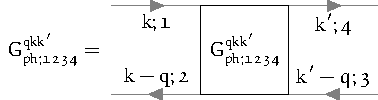
\includegraphics[scale=1.4]{../../Graphics/Diagrams/two_particle_green_channels/two_particle_green_channels_ph}}\vspace{0.5cm}\\
  \subfloat{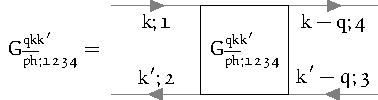
\includegraphics[scale=1.4]{../../Graphics/Diagrams/two_particle_green_channels/two_particle_green_channels_ph_bar}}\vspace{0.5cm}\\
  \subfloat{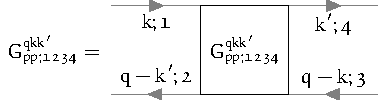
\includegraphics[scale=1.4]{../../Graphics/Diagrams/two_particle_green_channels/two_particle_green_channels_pp}}
  \caption{Two-particle Green's functions in the different frequency notations of \eqref{eq:ph_freq} - \eqref{eq:pp_freq} expressed in Feynman diagrams. The frequency notation is encoded in an additional subscript, $\{\text{ph}, \overline{\text{ph}},\text{pp}\}$.}
\end{figure}


\end{document}
